Este trabajo persigue implementar un algoritmo regresivo usando una DNN para predecir el momento transverso de muones de alto-$p_{T}$, intentando mejorar la asignaci\'on de $p_{T}$ proporcionada por los algoritmos actuales de CMS. \\

Puesto que parte de los problemas de reconstrucci\'on de este tipo de muones tiene que ver con la alta probabilidad de producci\'on de cascadas electromag\'eticas y por consiguiente la alta multiplicidad de segmentos en el sistema de muones, la propuesta tiene como elemento clave el estudio de la  distribuci\'on espacial de segmentos en las c\'amaras de muones. En particular, cada elemento del conjunto de datos utilizados en este estudio estar\'a compuesto por el $p_{T}$ proporcionado por el algoritmo TuneP, la informaci\'on de la traza del mu\'on reconstruida \'unicamente en el tracker, as\'i como sus extrapolaciones al sistema de muones, junto con informaci\'on acerca del n\'umero y distribuci\'on de los segmentos encontrados en torno a dichas extrapolaciones. \\

En la presente secci\'on se detallar\'an las herramientas y metodolog\'ia utilizadas para la extracci\'on y tratamiento de los datos.


\subsection{Herramientas utilizadas para el an\'alisis}\label{sec:tools}

Las herramientas utilizadas en este trabajo cumplen diversas funciones, pasando por la generaci\'on y simulaci\'on del paso de los muones por el detector, la reconstrucci\'on y obtenci\'on de las variables de inter\'es, y el posterior an\'alisis. En particular, pueden diferenciarse las siguientes herramientas:  

\begin{itemize}

\item Pythia~\cite{Sjstrand2008ABI} es un generador de Monte-Carlo que tiene como objetivo proporcionar todos los elementos necesarios para la simulaci\'on de eventos fruto de la colisi\'on de part\'iculas en condiciones de alta energ\'ia como las del LHC. Concretamente, se utilizar\'a Pythia para generar una muestra representativa de muones de alto momento de la que emerger\'an las muestras de entrenamiento y testeo de la DNN. Las macroinstrucciones usadas para la producci\'on de la muestra se pueden encontrar en el repositorio~\cite{generator}.

\item CMSSW~\cite{cmssw} es una colecci\'on de software abierto de la colaboraci\'on CMS basado en C++ y Pythia utilizado principalmente para la simulaci\'on, calibraci\'on, alineamiento, y reconstrucci\'on de objetos f\'isicos (como los muones a partir de sus segmentos y trazas). CMSSW a su vez utiliza Geant4~\cite{Agostinelli:2002hh}, que es el programa encargado de simular el comportamiento de las partículas a su paso por el detector. \\
Para este trabajo se ha creado un m\'odulo en C++ que puede encontrarse en \cite{analyzer}. Este c\'odigo utiliza diferentes herramientas de CMSSW para realizar la selecci\'on apropiada de muones y segmentos que se describir\'a en la subsecci\'on~\ref{sec:selection}. 

\item ROOT~\cite{root} es el marco de trabajo m\'as utilizado en f\'isica de altas energ\'ias para el procesado de datos, para an\'alisis estad\'istico, y para la visualizaci\'on y almacenamiento de los mismos. ROOT est\'a basado en programaci\'on orientada a objetos y escrito en C++, y se usar\'a como formato de los datos de entrada y salida del c\'odigo de selecci\'on~\cite{analyzer}, almacenando la informaci\'on recogida como objetos de ROOT.

\item Pandas~\cite{mckinney-proc-scipy-2010} (del ingl\'es \textit{Python Data Analysis Library}), es una librer\'ia de Python que ofrece gran rendimiento en el manejo de estructuras tabulares de datos. En este caso, se usar\'a Pandas, previa transformaci\'on de los datos en formato ROOT a formato de texto, para el procesado de los segmentos seleccionados (operaciones de limpiado de los datos, agregaciones, construcci\'on de las variables de entrenamiento...etc). Los m\'odulos creados para el procesado pueden encontrarse en \cite{processor}.

\item TensorFlow~\cite{tensorflow2015-whitepaper} es un librer\'ia de c\'odigo abierto desarrollada por Google que contiene la estructura matem\'atica de distintos algoritmos de aprendizaje autom\'atico como las redes neuronales artificiales. Se utilizar\'a TensorFlow para entrenar el modelo de regresi\'on al momento transverso de los muones.

\end{itemize}


La secuencia de trabajo en cuanto a las herramientas utilizadas se muestra esquem\'aticamente en la Figura~\ref{fig:diagram}.

\begin{center}
\smartdiagramset{border color=none,
   text width=3cm, font=\fontsize{10pt}{12pt}\selectfont,
   module x sep=4.0,     
   back arrow disabled=true}
\smartdiagram[flow diagram:horizontal]{
  Simulaci\'on de muones con Pythia y Geant4,
  Selecci\'on de muones y segmentos con CMSSW (salida en formato ROOT),
  Procesado de datos y construcci\'on de variables con Pandas,
  Entrenamiento de la red neuronal profunda usando TensorFlow.}
\captionof{figure}{Uso secuencial de las distintas herramientas utilizadas en el trabajo.}
\label{fig:diagram}        
\end{center}


\subsection{Muestra de simulaci\'on utilizada}\label{sec:sample}

Se han generado un total de 965000 sucesos de colisiones prot\'on-prot\'on a una energ\'ia de centro de masas de 13 TeV\footnote{condiciones actuales de funcionamiento del acelerador LHC} mediante simulaci\'on de Monte-Carlo utilizando el programa Pythia \cite{generator}, donde cada suceso contiene un \'unico mu\'on. \\
Se impone que los muones generados tengan un momento transverso aleatoriamente distribuido en el rango entre 20 y 2500 GeV y espacialmente repartidos en -2.5 $< \eta <$ 2.5, y se simula el paso de dichos muones por el detector CMS con el paquete Geant4. \\

La simulaci\'on de los procesos de colisi\'on es computacionalmente costosa y en general requiere del uso de clusters de ordenadores. El tama\~no de la muestra obtenida se ha considerado razonable teniendo en cuenta el tiempo de computaci\'on y el espacio de almacenamiento necesario. \\

En la Figura~\ref{fig:data_recopt_genpt} se muestra la distribuci\'on bidimensional del momento transverso dado por el algoritmo TuneP en funci\'on del momento transverso de generaci\'on para todos los muones de la muestra que pasan la selecci\'on detallada en la subsecci\'on~\ref{sec:selection}. \\

\begin{figure}[h!]
\centering
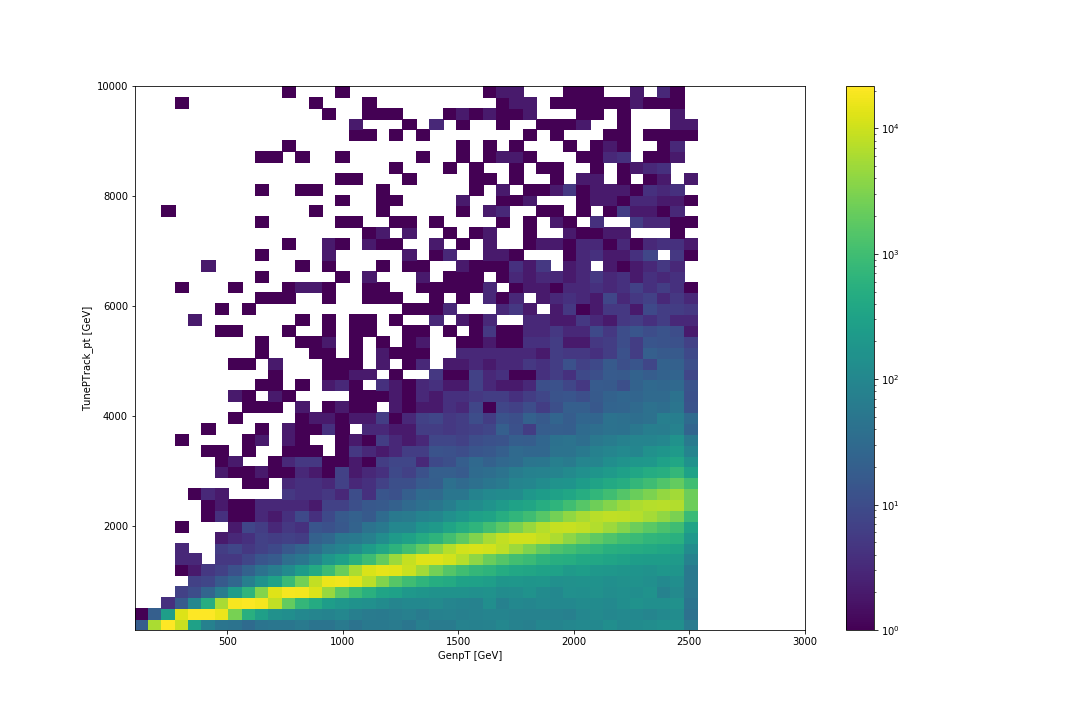
\includegraphics[width=1.0\textwidth]{figures/data_tunePpt_genpt.png}
\caption{Distribuci\'on bidimensional del $p_{T}$ proporcionado por el algoritmo TuneP en funci\'on del $p_{T}$ de generaci\'on para los muones de la muestra.}
\label{fig:data_recopt_genpt}  
\end{figure}



\subsection{Preparaci\'on del conjunto de datos: selecci\'on de muones y segmentos}\label{sec:selection}

El proceso de selecci\'on de los muones y segmentos, as\'i como de la producci\'on de las extrapolaciones (ver c\'odigo \cite{analyzer}) a partir de la muestra de simulaci\'on, consta de las siguientes partes: 

\begin{enumerate}

\item Lectura de datos: en los datos de entrada, los muones y segmentos reconstruidos por evento se almacenan en colecciones de ROOT, que funcionan a modo de contenedor de informaci\'on. Por tanto, el primer paso es leer las colecciones para poder iterar sobre ellas. 

\item Se recorre la colecci\'on de muones y se seleccionan aquellos que tengan una traza reconstruida en el tracker con $p_{T} >$ 200 GeV, y se requiere que esta traza est\'e pr\'oxima a la traza real generada del mu\'on dentro de un cono de radio $\Delta$R = $\sqrt{(\Delta\eta^{2}+\Delta\phi^{2})} <$  0.3. De esta forma se pretende garantizar que el mu\'on generado coincida exactamente con la traza considerada.

\item Posteriormente, se recorren las colecciones de segmentos encontradas en el suceso, y se almacenan sus coordenadas y los identificadores de los detectores en los que se encuentran en caso de que los segmentos sean v\'alidos\footnote{Que son compatibles con la trayectoria inicial de la traza, y con un $\chi$\textsuperscript{2} del ajuste de las se\~nales que componen el segmento no muy elevado.}, y sus coordenadas se hayan medido correctamente.

\item Se selecciona la posici\'on m\'as externa de la traza del tracker y se extrapola a la superficie de cada una de las c\'amaras de muones registradas donde se ha encontrado al menos un segmento. \\
El proceso de extrapolaci\'on se lleva a cabo utilizando un software especializado que integra la trayectoria de los muones aplicando la ley de Lorentz y teniendo en cuenta sus interacciones con el material de los detectores, como la ionizaci\'on o la dispersi\'on m\'ultiple Coulombiana.

\item De todos los segmentos guardados en el paso 3, se seleccionan aquellos que se encuentren en c\'amaras donde las extrapolaciones son v\'alidas (compatibles con la direcci\'on de la trayectoria inicial), vayan en la direcci\'on del campo magn\'etico impuesto por el solenoide de CMS, y cumplan que la distancia entre el centro de la c\'amara y la propia extrapolaci\'on no exceda el tama\~no propio de la c\'amara. Este \'ultimo requerimiento es de vital importancia, ya que las superficies a las que se extrapola son planos de dimensi\'on infinita (sin delimitar por las dimensiones reales de las c\'amaras), y una part\'icula cargada en movimiento sometida a un campo magn\'etico siempre puede cortar un plano de dimensi\'on infinita al curvarse.

\item Se guardan todas las variables de inter\'es como objetos de ROOT, es decir, la informaci\'on sobre la traza del mu\'on en el tracker, las coordenadas y direcciones de los segmentos recogidos, y las coordenadas de las extrapolaciones.
\end{enumerate}


En las Figuras~\ref{fig:segments_pos} y \ref{fig:props_pos} se muestran las posiciones espaciales de los segmentos y las propagaciones seleccionadas en los planos xy y xz. \\


\begin{figure}
\centering
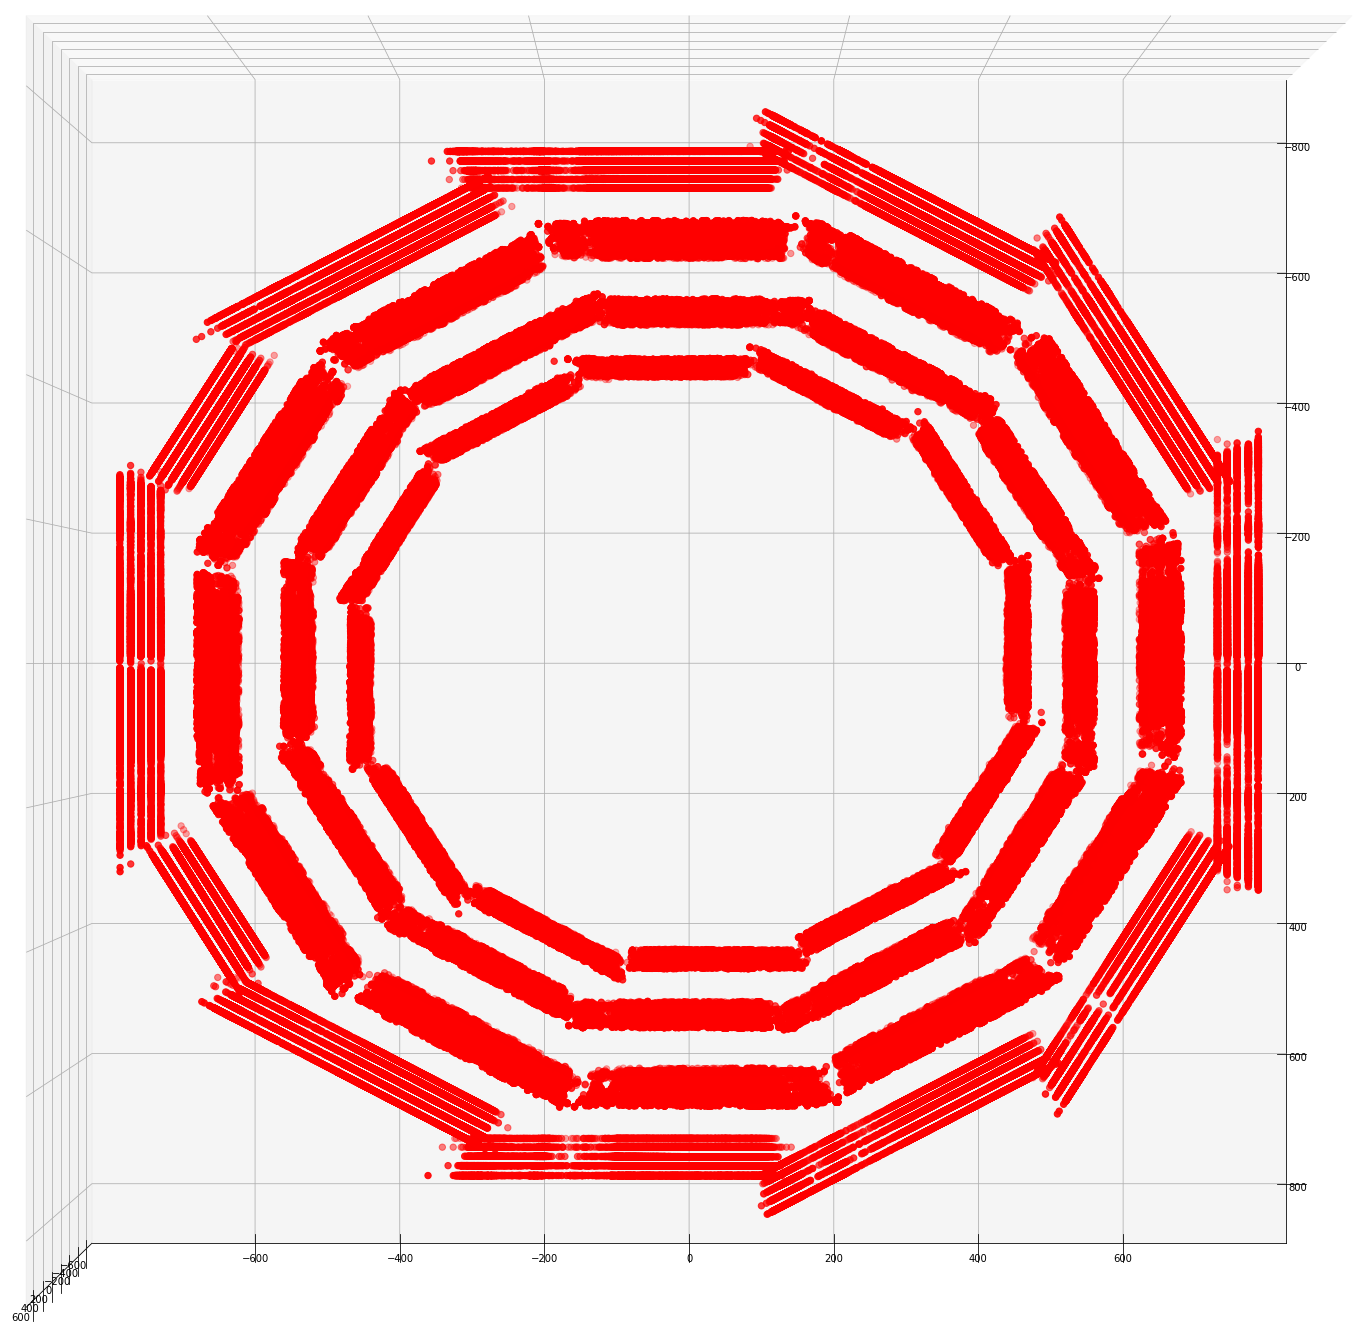
\includegraphics[width=0.4\textwidth]{figures/Hits_DT_xy.png}
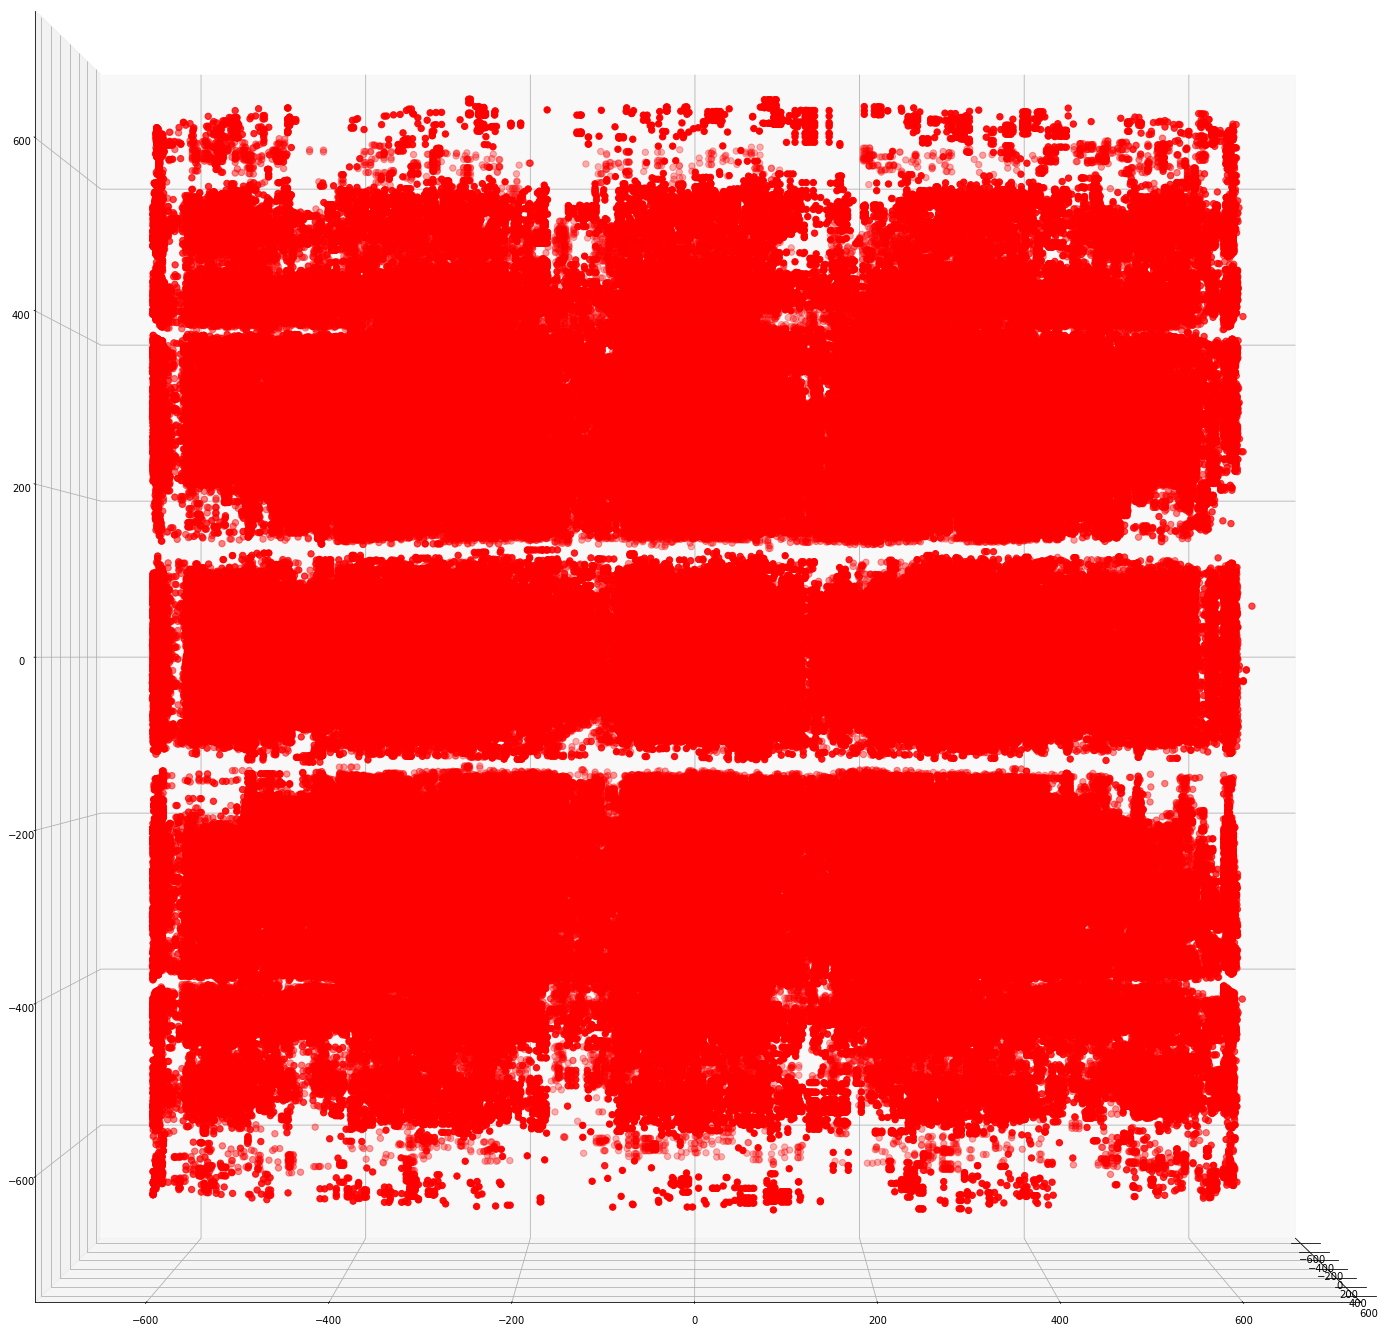
\includegraphics[width=0.4\textwidth]{figures/Hits_DT_xz.png}
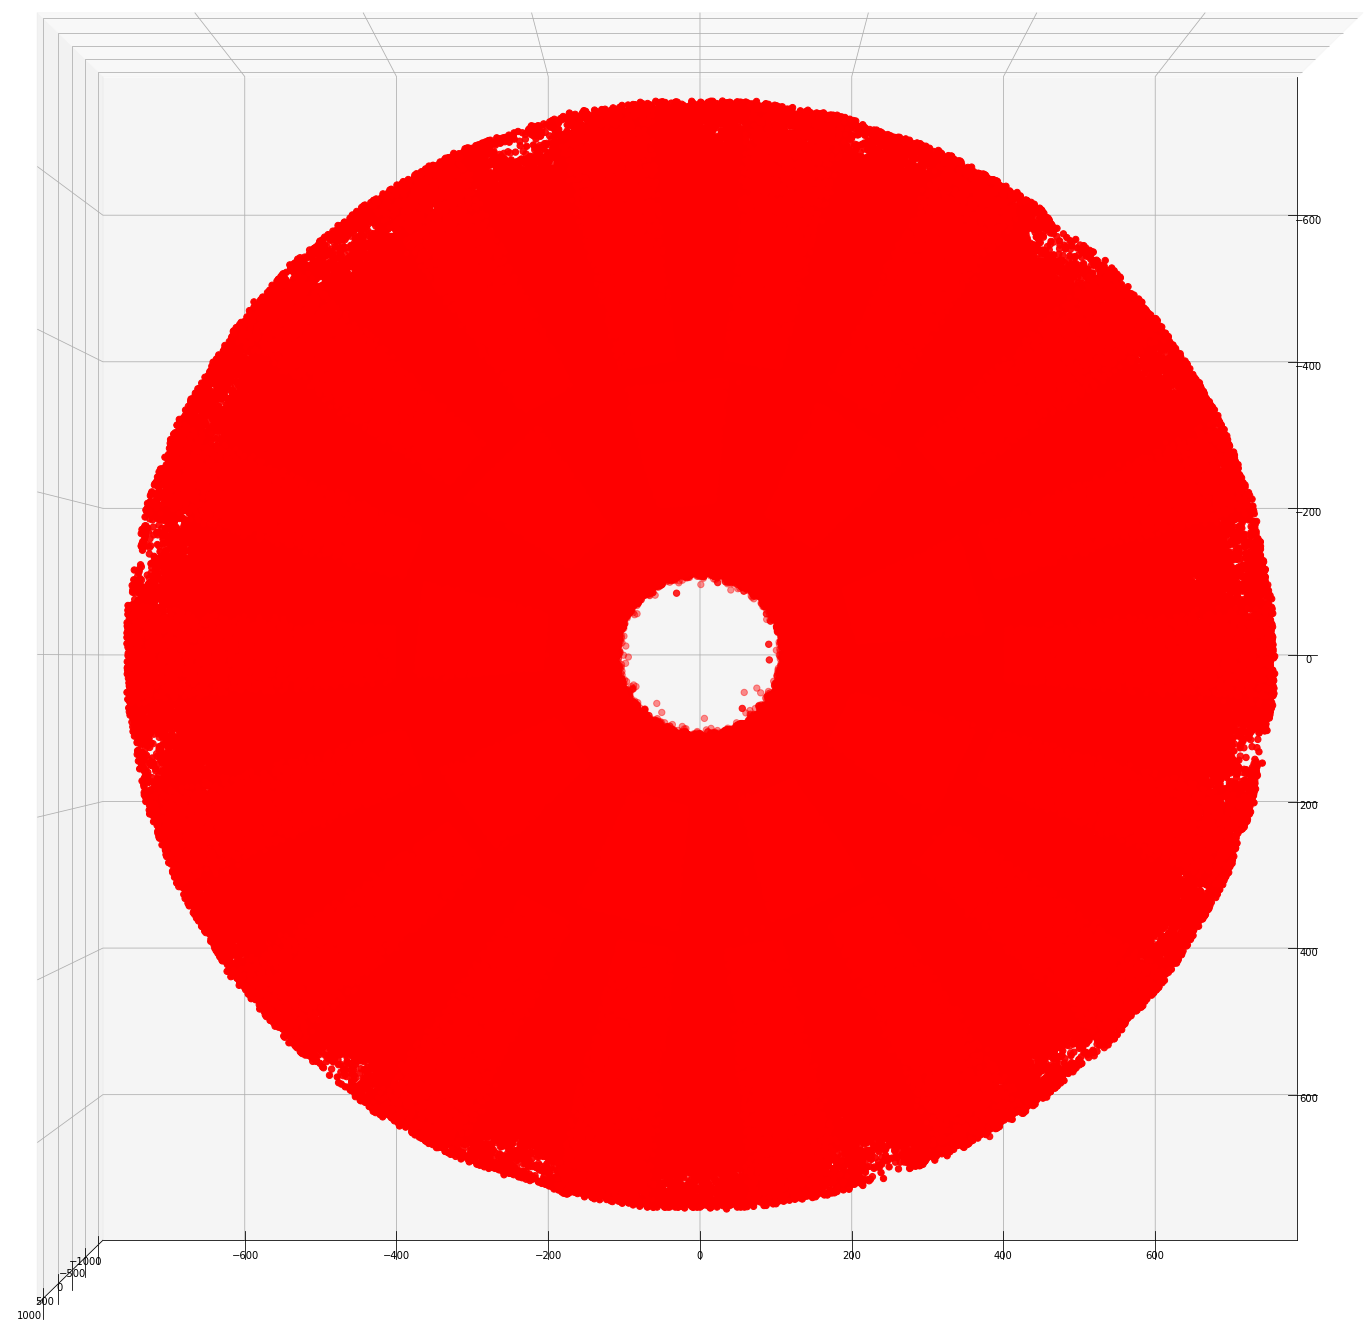
\includegraphics[width=0.4\textwidth]{figures/Hits_CSC_xy.png}
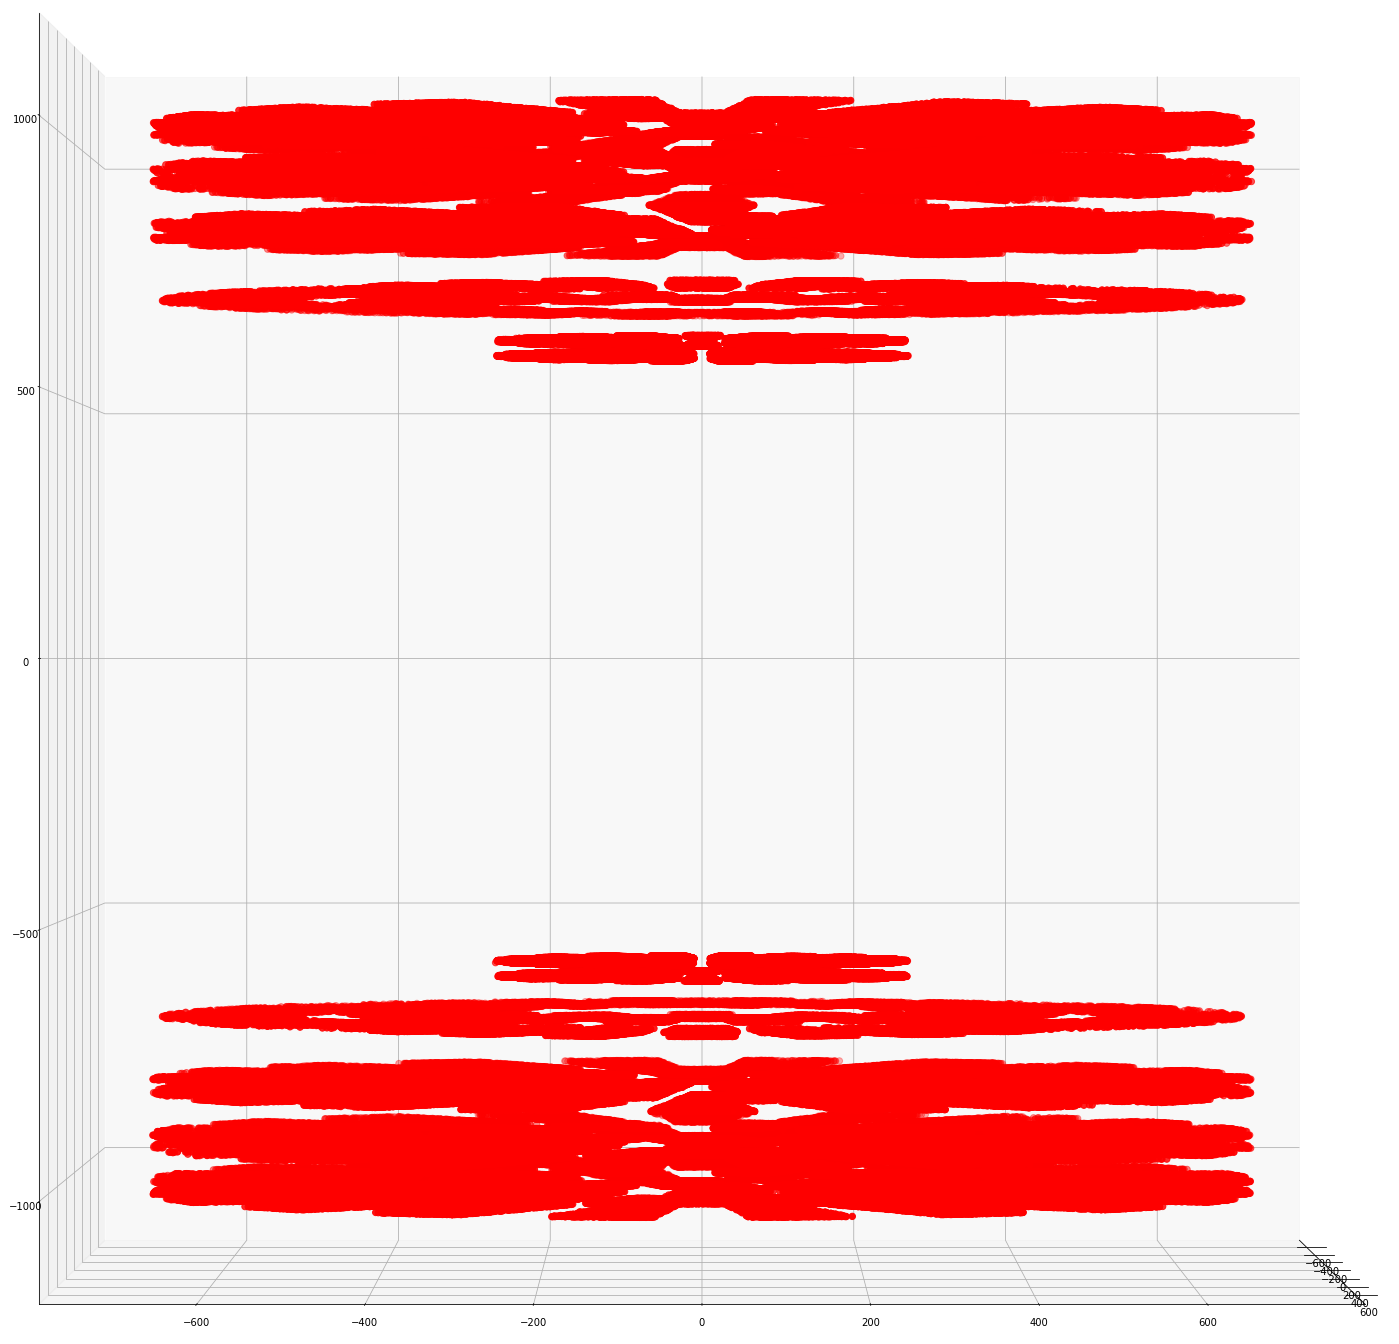
\includegraphics[width=0.4\textwidth]{figures/Hits_CSC_xz.png}
\caption{Posiciones geom\'etricas de todos los segmentos seleccionados. Arriba izquierda: Segmentos en DTs en el plano xy. Arriba derecha: Segmentos en DTs en el plano xz. Abajo izquierda: Segmentos en CSCs en el plano xy. Abajo derecha: Segmentos en CSCs en el plano xz.}
\label{fig:segments_pos}
\end{figure}


\begin{figure}
\centering
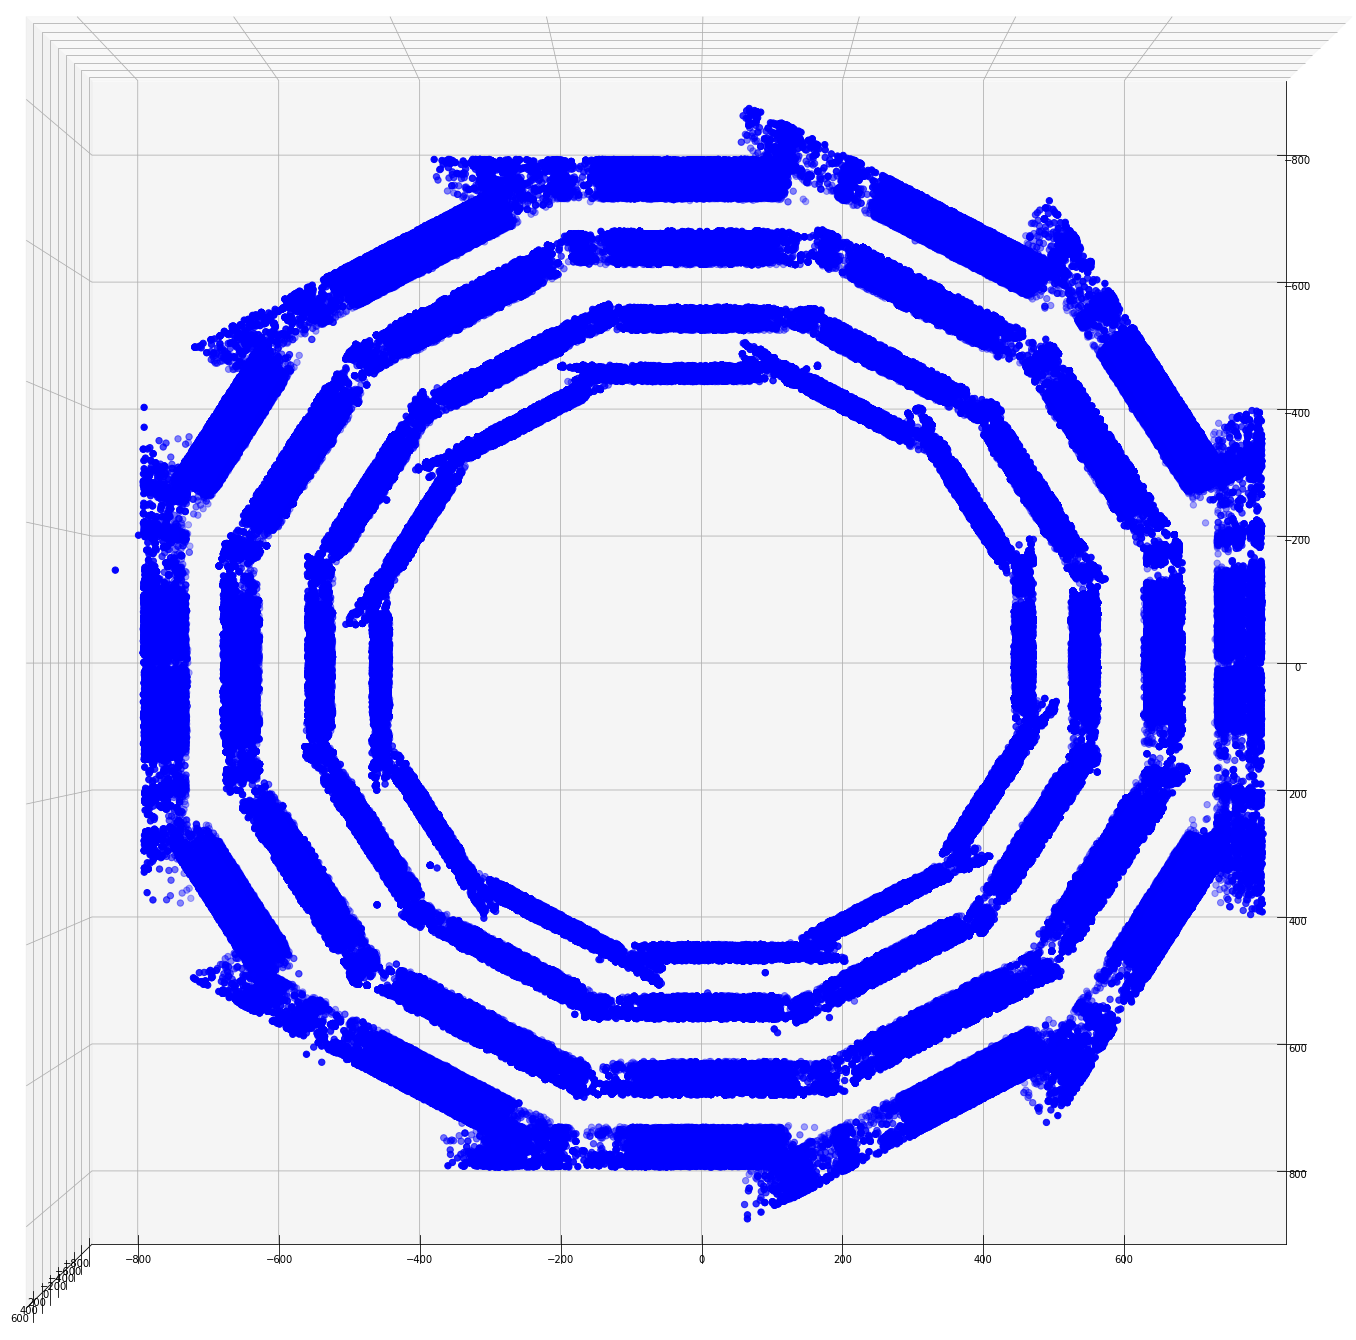
\includegraphics[width=0.4\textwidth]{figures/Props_DT_xy.png}
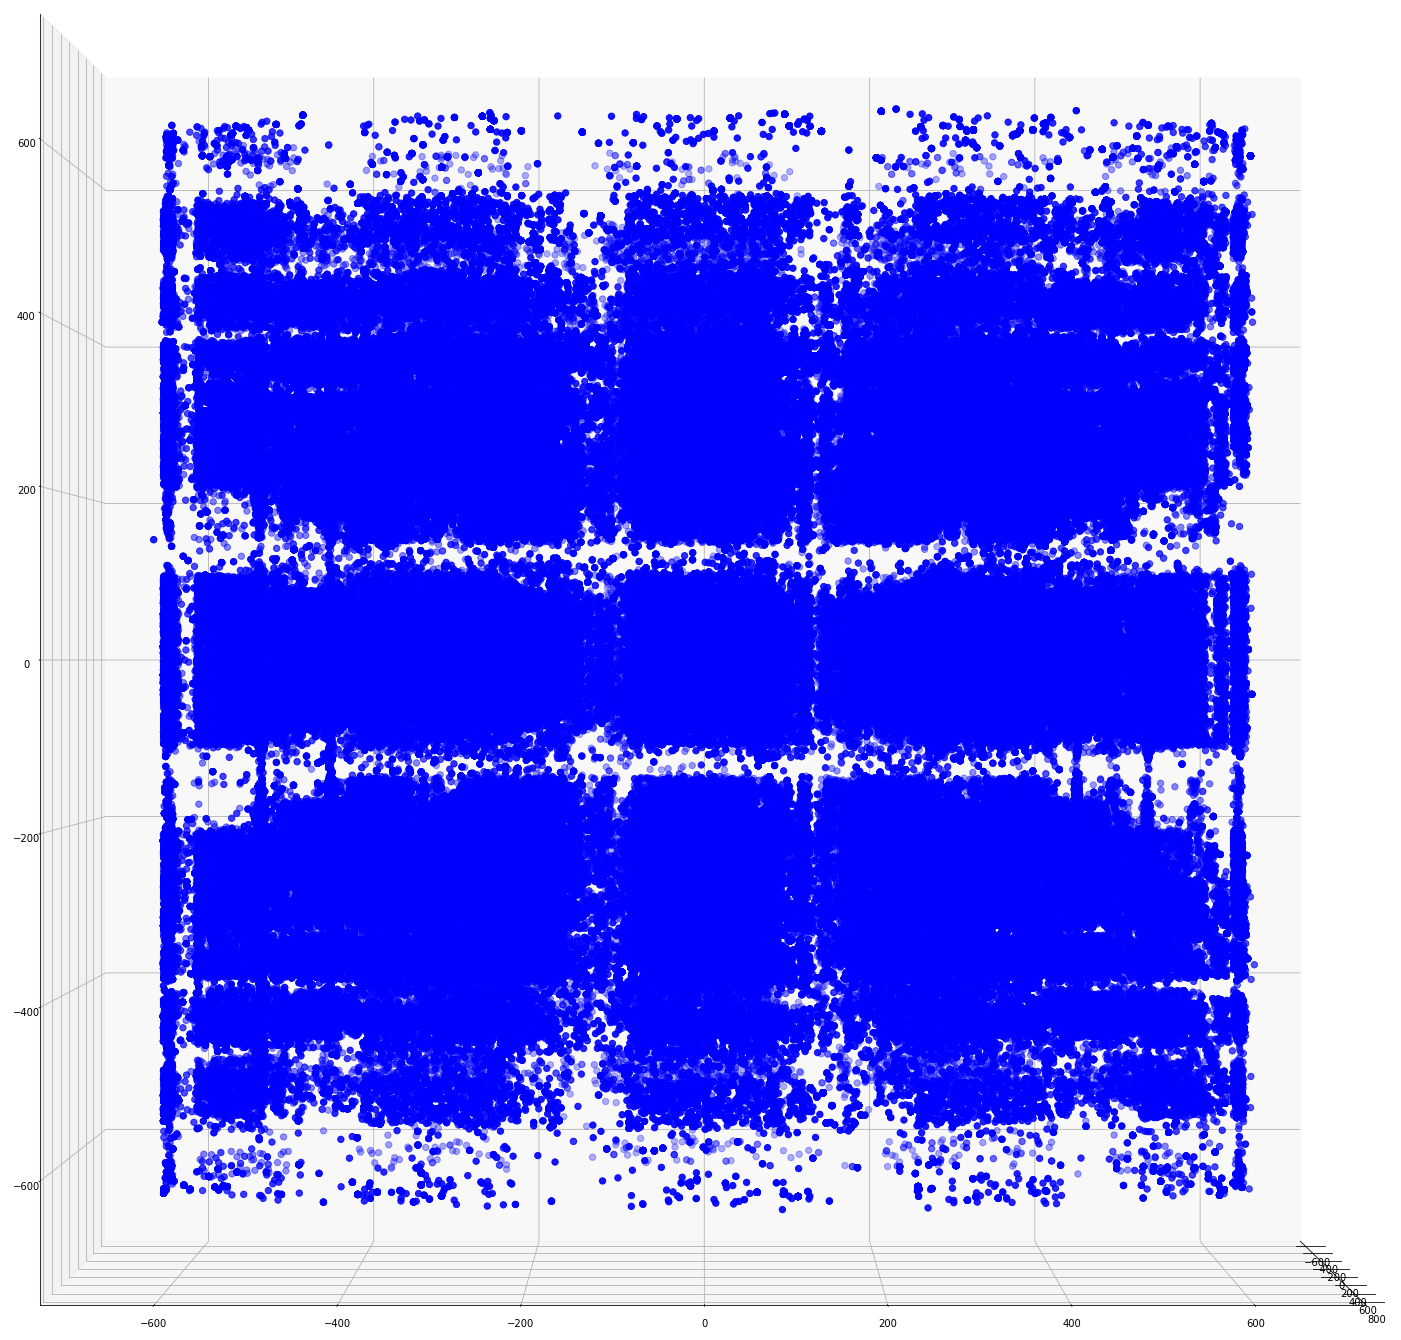
\includegraphics[width=0.4\textwidth]{figures/Props_DT_xz.png}
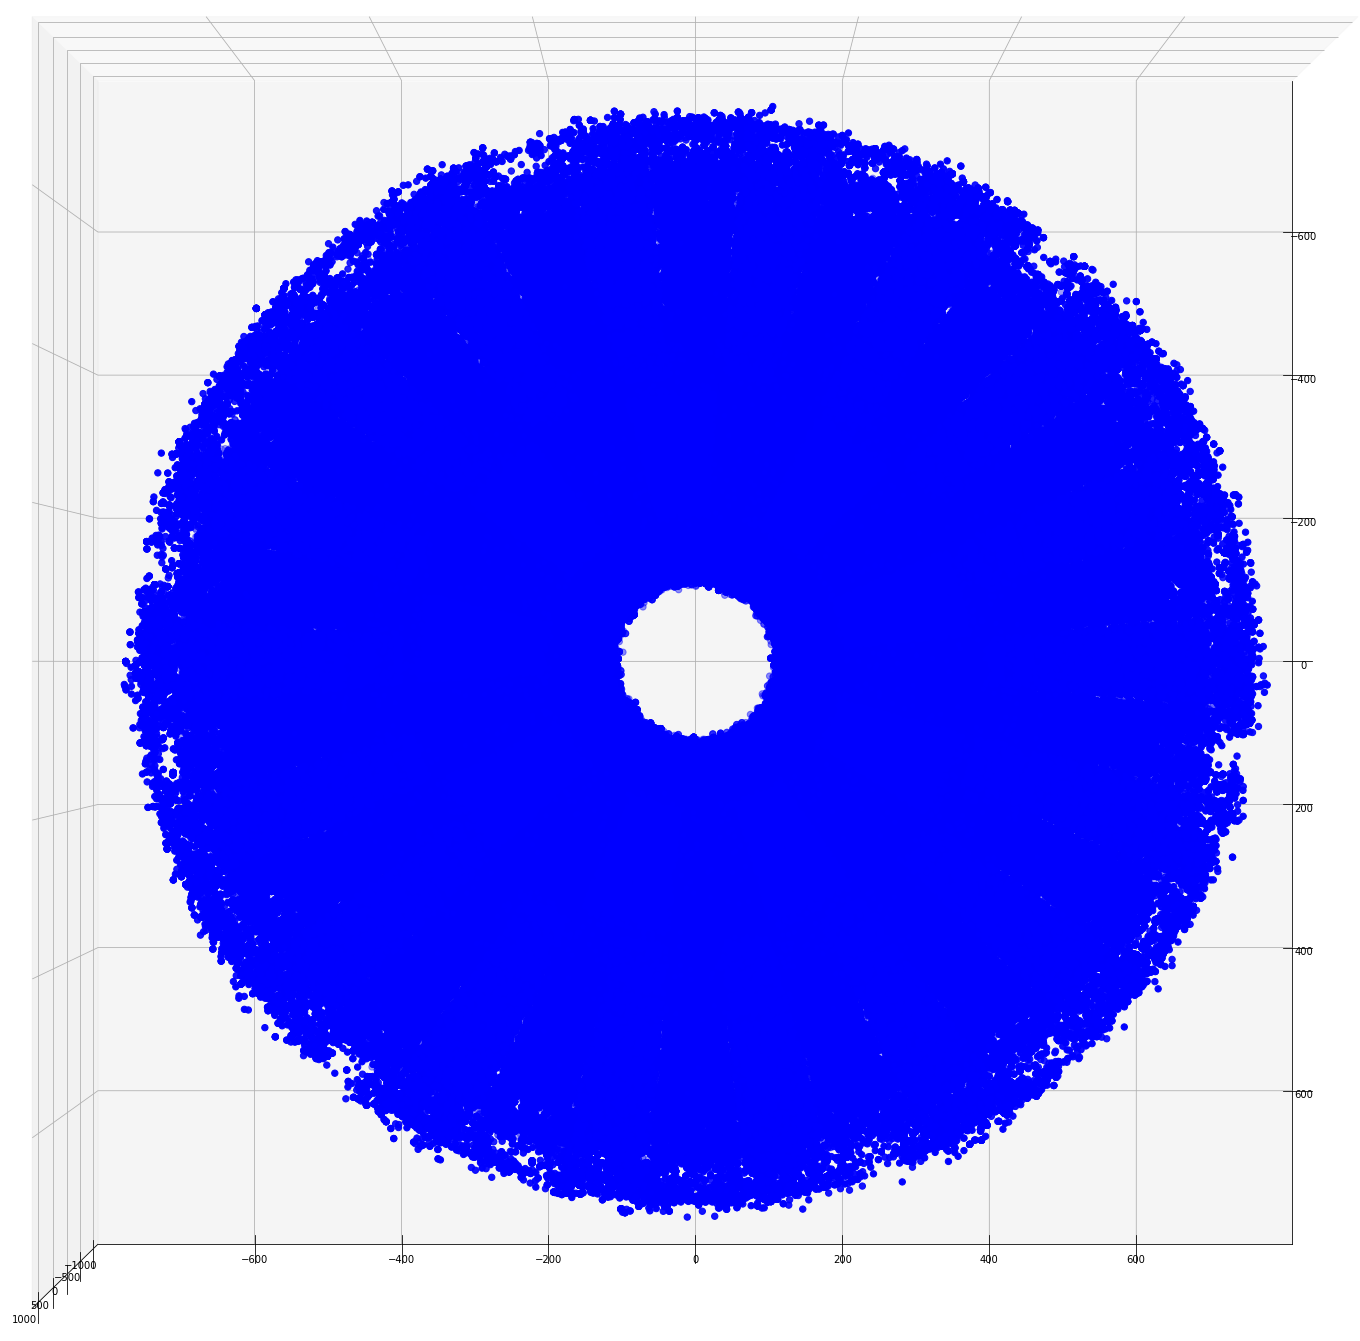
\includegraphics[width=0.4\textwidth]{figures/Props_CSC_xy.png}
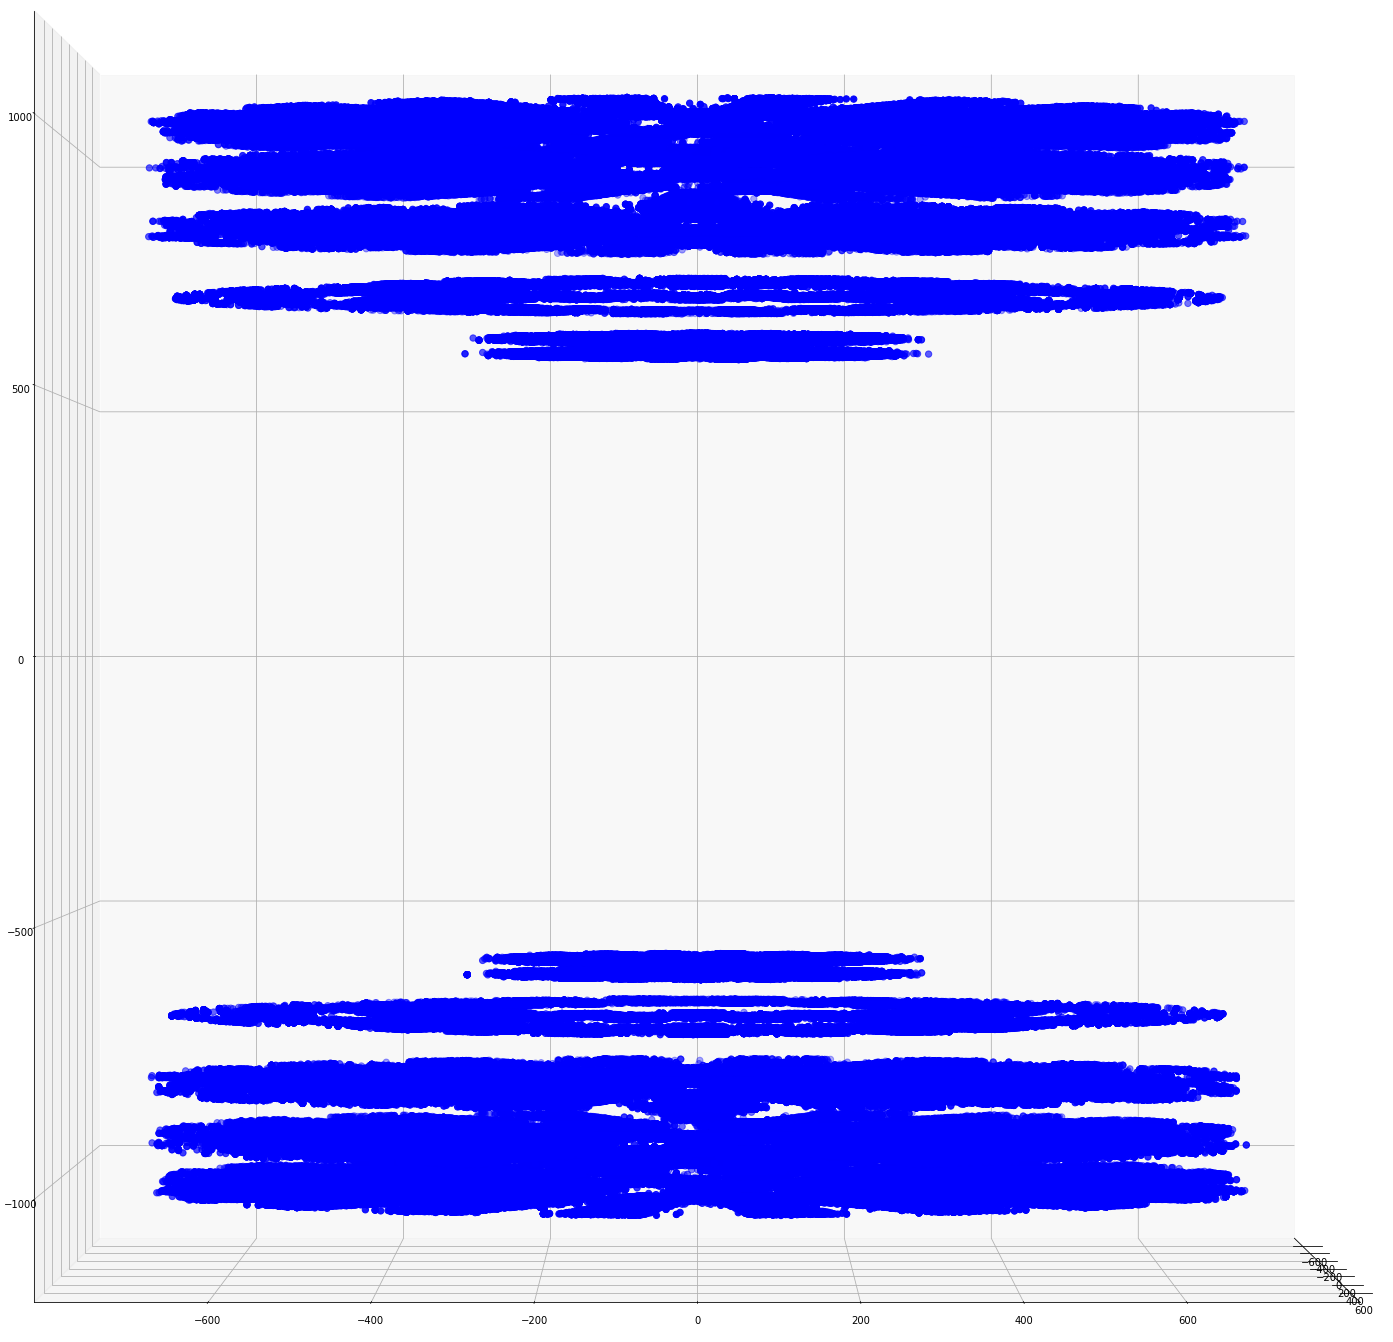
\includegraphics[width=0.4\textwidth]{figures/Props_CSC_xz.png}
\caption{Posiciones geom\'etricas de todos los propagaciones seleccionados. Arriba izquierda: Propagaciones en DTs en el plano xy. Arriba derecha: Propagaciones en DTs en el plano xz. Abajo izquierda: Propagaciones en CSCs en el plano xy. Abajo derecha: Propagaciones en CSCs en el plano xz.}
\label{fig:props_pos}
\end{figure}

Para la construcci\'on de las variables que ser\'an utilizadas en el entrenamiento de la DNN se usan agregaciones de Pandas (ver doStep1.py en \cite{processor}). As\'i, para cada mu\'on se agregan los segmentos encontrados en cada estaci\'on de DTs y CSCs y se obtiene el n\'umero total de segmentos por estaci\'on, la media espacial de la distribuci\'on de segmentos, su desviaci\'on est\'andar, la asimetr\'ia, y la kurtosis.



\subsection{Distribuciones de control}\label{sec:plots}

Tras la obtenci\'on de la muestra que ser\'a utilizada para el entrenamiento y testeo de la DNN, se han realizado varias comprobaciones para asegurar su calidad y coherencia. \\

En primer lugar, se seleccionan muones con cuatro o m\'as segmentos en las DTs o CSCs, y se exige que estos tengan al menos un segmento en cada estaci\'on. Esta submuestra contiene trazas de muones que pueden considerarse completas. \\
Posteriormente, se separan los muones que cumplan estas condiciones en dos categor\'ias: aquellos que tienen exactamente cuatro segmentos (uno en cada estaci\'on), y aquellos que tienen m\'as de cuatro segmentos, de forma que los muones pertenecientes a la segunda categor\'ia son susceptibles de haber emitido una cascada electromagn\'etica. De esta manera, si para cada mu\'on se selecciona el m\'aximo valor de distancia entre el segmento y la extrapolaci\'on de entre todos los pares segmento-extrapolaci\'on que lo componen, uno esperar\'ia encontrar valores relativamente bajos en la primera categor\'ia, y valores m\'as altos en la segunda, debido a la presencia de segmentos adicionales. \\
Las distribuciones para ambos grupos se muestran en la Figura~\ref{fig:data_dist}. \\

\begin{figure}[h]
\centering
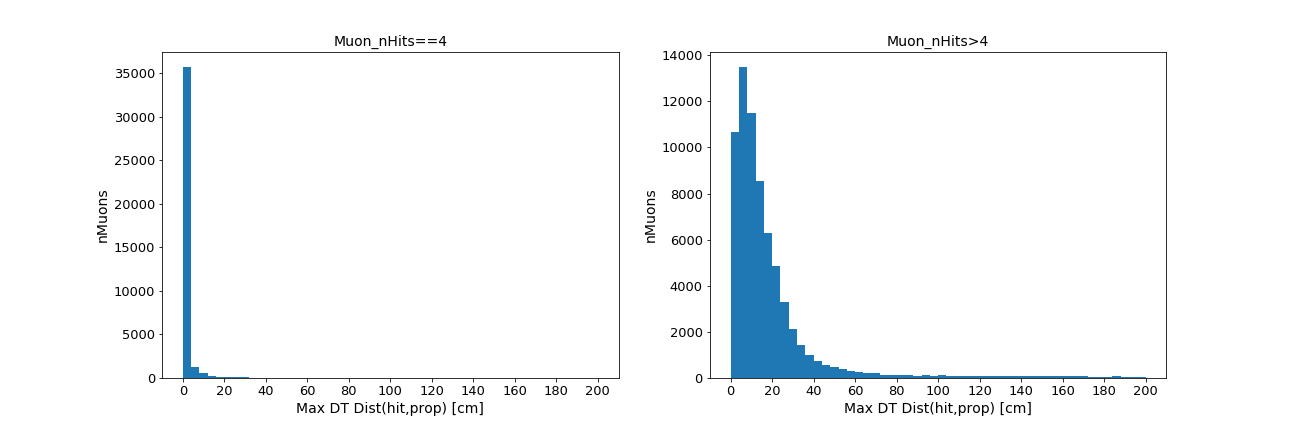
\includegraphics[width=1.1\textwidth]{figures/data_simple_DT_dist.png}
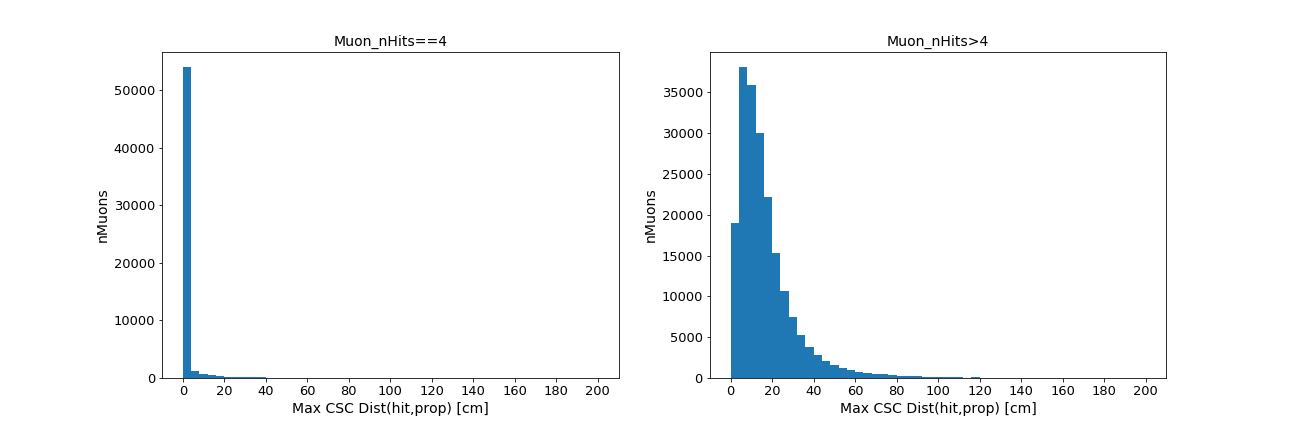
\includegraphics[width=1.1\textwidth]{figures/data_simple_CSC_dist.png}
\caption{Distribuciones del m\'aximo valor encontrado de distancia entre el segmento y la extrapolaci\'on (por mu\'on). Arriba izquierda: Muones con cuatro segmentos en las DTs, uno en cada estaci\'on. Arriba derecha: Muones con m\'as de cuatro segmentos en las DTs, y con al menos un segmento por estaci\'on. Abajo izquierda: Muones con cuatro segmentos en las CSCs, uno en cada estaci\'on. Abajo derecha: Muones con m\'as de cuatro segmentos en las CSCs, y con al menos un segmento por estaci\'on.}
\label{fig:data_dist}        
\end{figure}


Por otra parte, en la Figura~\ref{fig:data_nSegmentsMean} se muestra la dependencia de la media del n\'umero de segmentos producidos por cada mu\'on con el $p_{T}$ de generaci\'on para todos los muones del conjunto de datos. Se observa en este caso que hay una clara tendencia ascendente del promedio del n\'umero de segmentos con el $p_{T}$, ya que como se indic\'o en la secci\'on~\ref{sec:intro}, a mayor $p_{T}$ mayor es la probabilidad de que el mu\'on emita una cascada y se encuentren por tanto m\'as se\~nales en las c\'amaras de muones.\\

Equivalentemente, en la Figura~\ref{fig:data_nShowersMean_genpt} se muestra la dependencia del promedio del n\'umero de cascadas encontradas por mu\'on con el $p_{T}$ de generaci\'on, donde el n\'umero de cascadas se define por mu\'on como el n\'umero de veces que se tienen m\'as de 20 se\~nales\footnote{N\'umero arbitrario de se\~nales que puede dar un indicio de que una cascada ha tenido lugar.} en alguna de las estaciones de DTs o CSCs. \
De nuevo se observa la tendencia ascendente acorde con lo esperado. \\



\begin{figure}[h!]
\centering
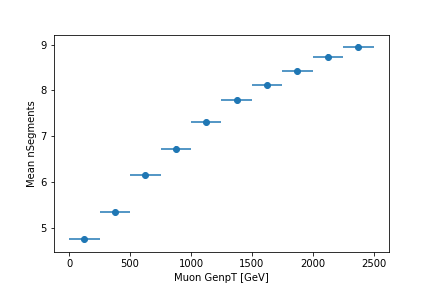
\includegraphics[width=0.45\textwidth]{figures/data_genpt_DT_MeanNSegments.png}
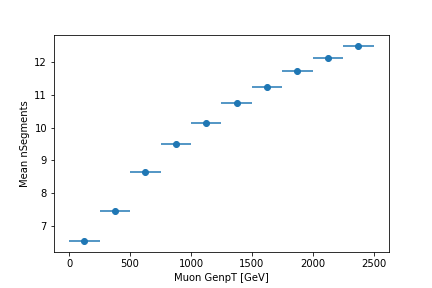
\includegraphics[width=0.45\textwidth]{figures/data_genpt_CSC_MeanNSegments.png}
\caption{Valor medio de segmentos encontrados por mu\'on en funci\'on del momento transverso generado, donde la incertidumbre en el eje de abscisas se corresponde con la desviación est\'andar de la distribuci\'on del n\'umero de segmentos por bin de $p_{T}$ dividida entre la ra\'iz cuadrada del n\'umero de muones en cada bin. Izquierda: Segmentos en las DTs. Derecha: Segmentos en las CSCs.}
\label{fig:data_nSegmentsMean}        
\end{figure}

\begin{figure}[h!]
\centering
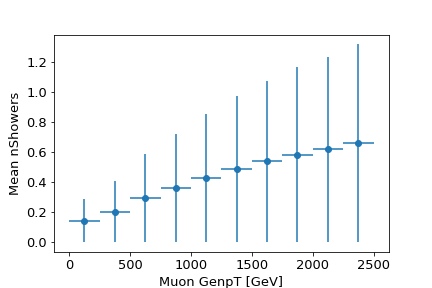
\includegraphics[width=0.45\textwidth]{figures/data_genpt_DT_MeanNshowers.png}
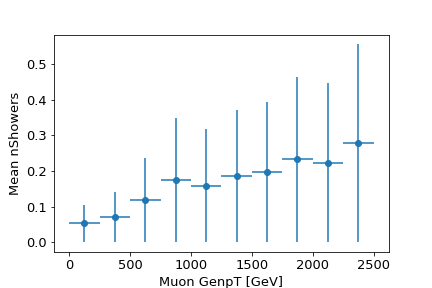
\includegraphics[width=0.45\textwidth]{figures/data_genpt_CSC_MeanNshowers.png}
\caption{Valor medio del n\'umero de cascadas en funci\'on del momento transverso generado, donde la incertidumbre en el eje de abscisas se corresponde con la desviación est\'andar de la distribuci\'on del n\'umero de cascadas por bin de $p_{T}$ dividida entre la ra\'iz cuadrada del n\'umero de muones en cada bin. Izquierda: Promedio de cascadas por mu\'on en las DTs. Derecha: Promedio de cascadas por mu\'on en las CSCs.}
\label{fig:data_nShowersMean_genpt}        
\end{figure}

\clearpage

Por \'ultimo, en la Figura~\ref{fig:data_R_genpt} se muestra la dependencia de la desviaci\'on est\'andar y del promedio de $R$~\eqref{eq:R} con el $p_{T}$ de generaci\'on para los muones detectados en las DTs ($\lvert \eta \rvert <$ 0.9). Puede observarse que la asignaci\'on de momento transverso se va degradando con el $p_{T}$ seg\'un lo esperado. \\

\begin{figure}[h!]
\centering
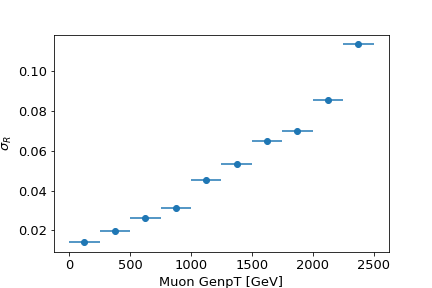
\includegraphics[width=0.45\textwidth]{figures/data_genpt_DT_sigmaR.png}
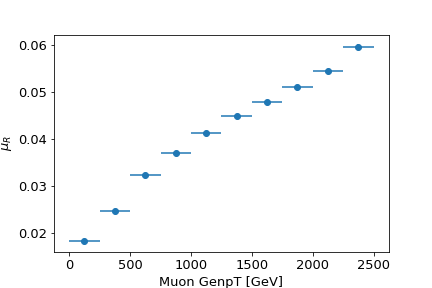
\includegraphics[width=0.45\textwidth]{figures/data_genpt_DT_R.png}
\caption{Dependencia de la desviaci\'on est\'andar y del valor medio de $R$ con el $p_{T}$ de generaci\'on para muones con $\lvert \eta \rvert <$ 0.9. Izquierda: Desviaci\'on est\'andar de $R$ en el eje de abscisas. Derecha: Valor medio de R en funci\'on en el eje de abscisas, donde la incertidumbre se corresponde con la desviación est\'andar de la distribuci\'on de R por bin de $p_{T}$ dividida entre la ra\'iz cuadrada del n\'umero de muones en cada bin.}
\label{fig:data_R_genpt}        
\end{figure}


\clearpage


 
